\documentclass[a4paper,14pt]{article}

\usepackage[utf8]{inputenc}
\usepackage[english]{babel}
\usepackage{graphicx, array, blindtext}
\usepackage[colorinlistoftodos]{todonotes}

\usepackage{enumitem}
\usepackage{amsmath}
\usepackage{amsthm}

\usepackage{nameref}
\usepackage{amssymb}
\usepackage{xcolor}
\usepackage{floatrow}
\usepackage{cancel}
\usepackage{fancyhdr}
\usepackage{graphicx}
\usepackage{verbatim}
\usepackage[document]{ragged2e}

\rhead{CS765 Assignment 3}
\usepackage{subcaption}
\usepackage{listings}


\usepackage{hyperref}

\begin{document}
\centering{

\title{\fontsize{150}{60}{CS765 Assignment 3}}

\author{
Prathamesh Pilkhane\\
Shashwat Garg \\
Vedang Asgaonkar}
}

\date{Spring 2023}
\maketitle

\justifying

% \tableofcontents
% \newpage

\justifying

\section*{Introduction}

Hello and Welcome to our CS765 Assignment 3. Here we implement a Dapp using Solidity, Ganache and Truffle.

\section{Code Flow}

\verb|client.py| uses python library \verb|web3| to connect to the ganache server. It calls the respective functions which have been implemented in solidity.\\\\
We use the python library \verb|networkx| to create a power-law degree distribution graph. It uses the Holme and Kim algorithm for growing graphs with powerlaw degree distribution.\\\\
We adjust the gas limit so as to remove the gas limit exceeded errors, both in \verb|client.py| as well as \verb|Payment.sol|\\\\
The remaining code in \verb|client.py| is simply just calling the required functions and storing the result values of the \verb|sendAmount| function.\\\\
In \verb|Payment.sol|, we implement the required 4 functions. Except \verb|sendAmount|, all others are pretty simple functions. In \verb|sendAmount|, we just need to implement a BFS in solidity, so it just costs a lot more in gas payments.



\section{Observation}

\subsection{Success Rate}

We do not observe very strong trends, but across various runs, the probability of success seems to go down as time progresses.\\
This can be attributed to the fact that we start from a very stable situation, and random transactions increase the randomness in the system.\\
Initially, whenever path exists, a transaction can pass through. Later, since we only look at the shortest path, there might be a case that shortest path can not transfer any more coins in that direction.\\\\
The intuition for the above is that even though there is no trend in the random sendAmount() calls, there are increasing number of situations possible where failure might occur, and thus, we expect the success rate to go down slightly.\\
Of course, the simple solution is to settle the contract and start afresh. Or with people entering and exiting the graph, this would also prevent the graph from getting lopsided edges.\\
As for the results, they are given below\\\\
\begin{table}[h!]
    \centering
    \caption{Success rate across runs}
    \label{tab:data}
    \begin{tabular}{|c|c|c|c|}
      \hline
      Txns & 10 & 5 & 3 \\
      \hline
      100 & 95 & 90 & 82 \\
      200 & 95 & 87 & 80 \\
      300 & 83 & 79 & 73 \\
      400 & 72 & 70 & 75 \\
      500 & 87 & 81 & 62 \\
      600 & 88 & 73 & 72 \\
      700 & 91 & 66 & 73 \\
      800 & 86 & 67 & 56 \\
      900 & 83 & 66 & 60 \\
      1000 & 84 & 75 & 65 \\
      \hline
    \end{tabular}
\end{table}
  
\begin{center}
    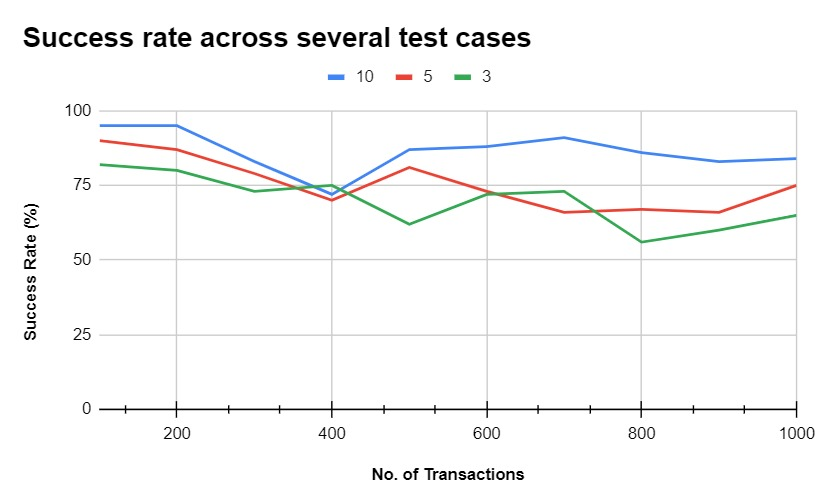
\includegraphics[width=10cm]{success_rate.jpeg}\\
\end{center}


\end{document}